\section{Resultados y Discusión}



% ---------------------------------------------------------
% 5. Efecto túnel cuántico: Crank–Nicolson
% ---------------------------------------------------------


\subsection{Resultados y Análisis: Efecto Túnel Cuántico}


\begin{figure}[h]
    \centering
    \href{https://youtu.be/dDUh9E-eRjU}{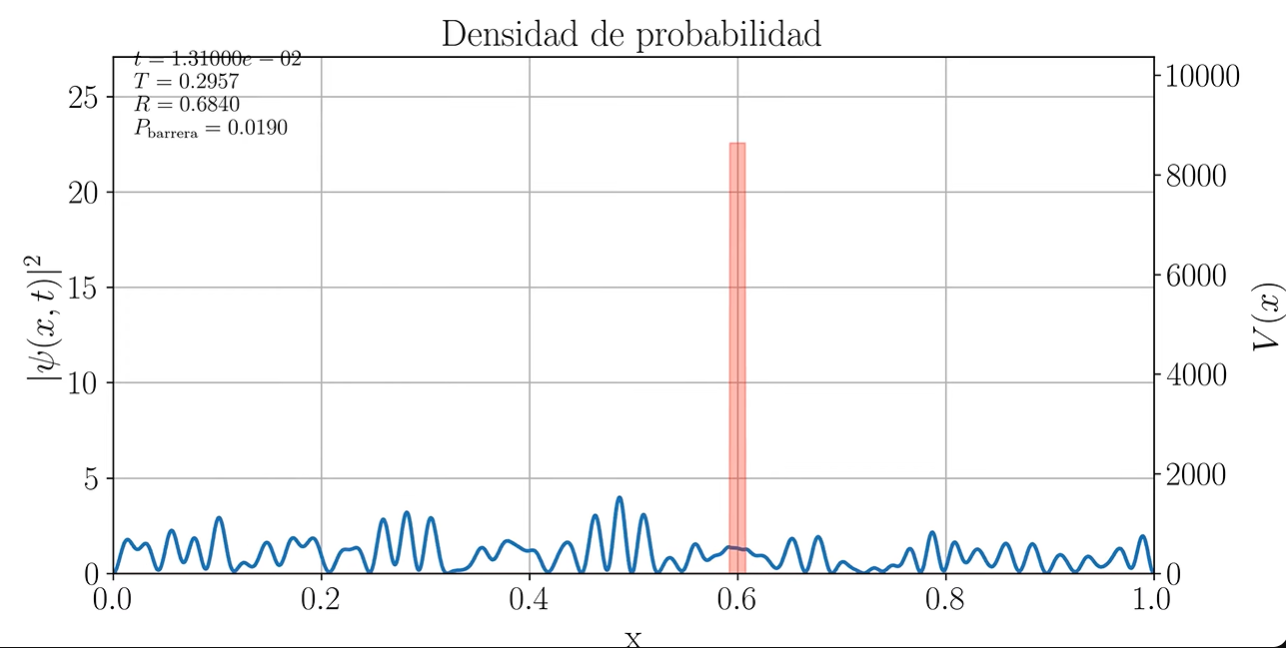
\includegraphics[width=0.75\linewidth]{figures/tunel_schrodinger.png}}
    \caption{Evolución temporal de la función de onda de un paquete gaussiano incidente sobre una barrera rectangular de potencial en el régimen \(V_0>E\). Animación completa disponible en \href{https://youtu.be/dDUh9E-eRjU}{YouTube}.}
    \label{fig:tunel_schrodinger}
\end{figure}


La simulación resuelve numéricamente la ecuación de Schrödinger unidimensional dependiente del tiempo mediante el esquema implícito de Crank–Nicolson. El sistema consiste en un paquete de ondas gaussiano inicialmente localizado en \(x_0=0.20\), propagándose con momento medio \(k_0=120\) hacia una barrera rectangular de altura \(V_0\) y anchura \(w\), centrada en \(x_c=0.60\).

La Figura \ref{fig:tunel_schrodinger} muestra la evolución temporal de la densidad de probabilidad \(|\psi(x,t)|^2\). Antes de alcanzar la barrera, el paquete mantiene una estructura gaussiana coherente y un perfil aproximadamente simétrico. Durante la interacción con la región potencial, la función de onda se divide dinámicamente en dos componentes: una fracción reflejada que se propaga hacia la izquierda y una fracción transmitida que emerge al otro lado de la barrera pese a verificarse el régimen clásico prohibido \(V_0>E\).

Por otro lado, la simulación registra la evolución temporal de las probabilidades integradas de transmisión \(T(t)\), reflexión \(R(t)\) y ocupación transitoria de la barrera \(P_{\mathrm{barrera}}(t)\). Los resultados constituyen una manifestación explícita del efecto túnel cuántico, fenómeno estrictamente prohibido en mecánica clásica.

Es decir, la atenuación que sufre la onda no implica la anulación completa de su amplitud, permitiendo una probabilidad finita de transmisión incluso en regiones clásicamente inaccesibles. Este comportamiento se ve reflejado en la Figura \ref{temporal} ya que la transmisión no permanece nula tras el primer encuentro de la onda con la barrera alrededor de $t\approx2.5\cdot10^{-3}s$, además, se verifica la estabilidad numérica del método debido a la conservación de la probabilidad dada por la Ecuación \ref{eq:conservacion_prob}. Este hecho comprueba que el algoritmo implementado respeta la unitariedad de la dinámica cuántica y valida el uso del método de Crank–Nicolson como herramienta robusta para estudiar fenómenos de transporte cuántico, dispersión resonante y propagación coherente en nanoestructuras potenciales.

\begin{figure}[H]
    \centering
    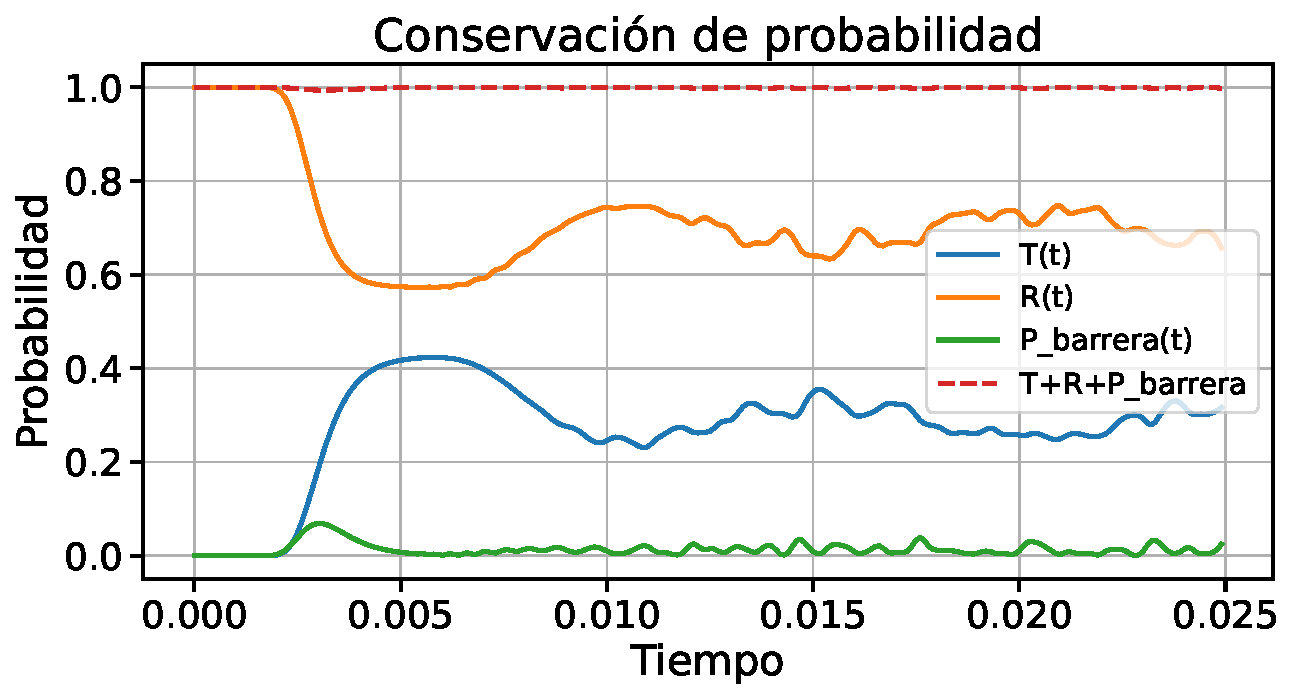
\includegraphics[width=0.7\textwidth]{figures/conservacion_probabilidad.pdf}
    \caption{Figura que muestra $R(t)$, $T(t)$, $P_{barrera}(t)$ así como $R(t)+T(t)+P_{barrera}(t)$.}
    \label{temporal}
\end{figure}

Por completitud, el primer pico de transmisión obtenido mediante Crank-Nicolson se puede comparar con la solución analítica, dada por la Expresión \ref{eq:T_analitica}, mostrando una similitud considerable en los resultados, con una desviación del 3\% ($T_{CN}^{max}=0.423,T_{an}=0.409)$. La correlación de estos resultados no es crítica para la veracidad de la simulación debido a que la fórmula analítica se obtiene en el caso de una onda plana que se propaga libremente hasta la barrera y tras atravesarla recupera su libertad de movimiento, pero su parecido sirve como una estimación para ratificar el buen funcionamiento del método.

Adicionalmente, se realizaron barridos paramétricos tanto en la altura del potencial \(V_0\) como en la anchura \(w\), obteniendo mapas bidimensionales \(T(V_0,t)\) y \(T(w,t)\), así como las transmisiones medias temporales \(\langle T \rangle\). Como se puede observar en la Figura \ref{fig:barridos}, el barrido paramétrico en $V_0$, evidencia que la transmisión decrece conforme aumenta la altura de la barrera, ya que el vector de decaimiento evanescente \(\kappa\) se incrementa y reduce la penetración efectiva de la función de onda. Por otro lado, el análisis respecto a la anchura \(w\) revela que pequeñas variaciones de grosor producen reducciones exponenciales de \(\langle T \rangle\). Este comportamiento reproduce directamente la predicción de la aproximación WKB, donde $T \sim e^{-2\kappa w}$.

\begin{figure}[H]
    \centering

    \begin{subfigure}[b]{0.42\textwidth}
        \centering
        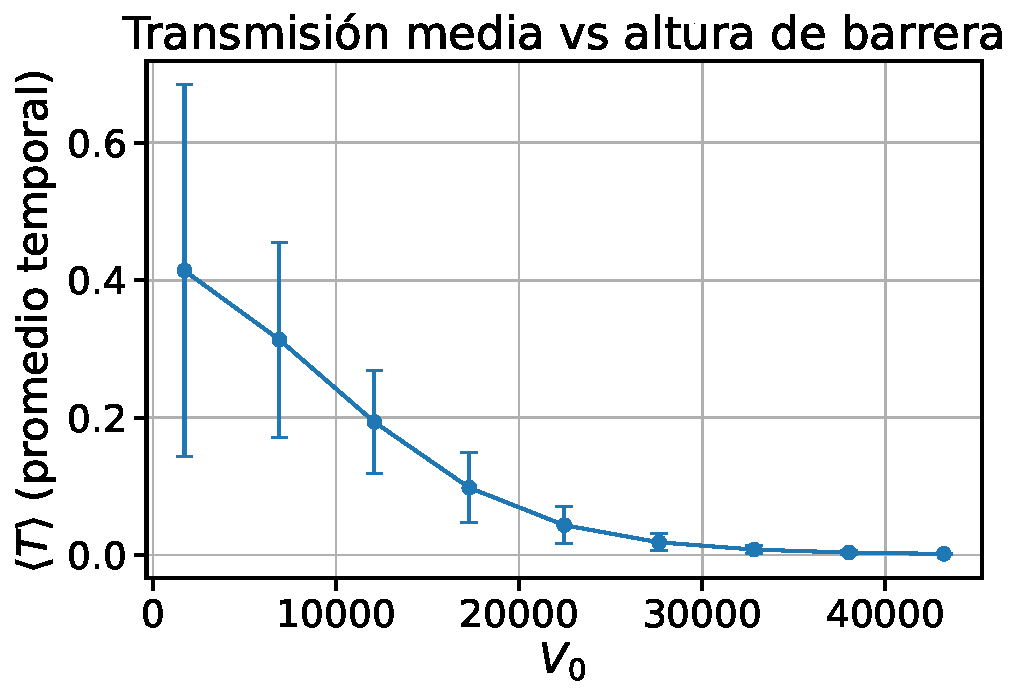
\includegraphics[width=\textwidth]{figures/T_medio_vs_V0.pdf}
        \caption{}
        \label{fig:barrido_V}
    \end{subfigure}
    \hfill
    \begin{subfigure}[b]{0.42\textwidth}
        \centering
        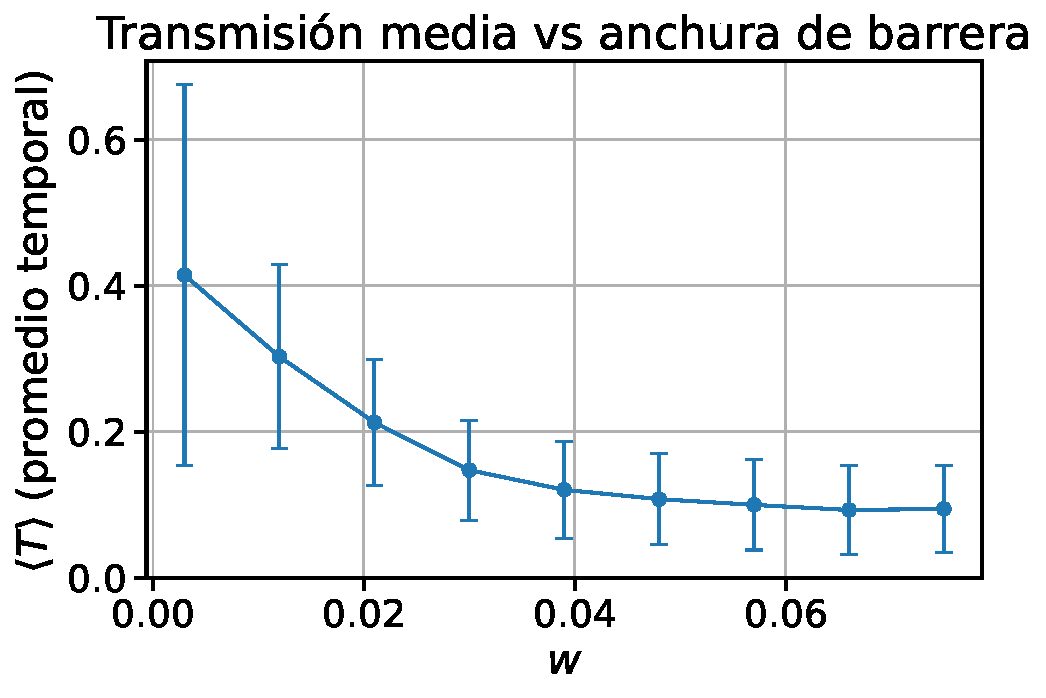
\includegraphics[width=\textwidth]{figures/T_medio_vs_w.pdf}
        \caption{}
        \label{fig:barrido_w}
    \end{subfigure}

    \caption{(a) Resultados del barrido para determinar $\langle T(V_0)\rangle_t$. (b) Resultados del barrido para determinar $\langle T(w)\rangle_t$}
  \label{fig:barridos}
\end{figure}

Otra forma de visualizar estos mismos resultados es un mapa que muestra $T(V_0,t)$ y $T(w,t)$, como se observa en la Figura \ref{fig:mapas}.

\begin{figure}[H]
    \centering

    \begin{subfigure}[b]{0.48\textwidth}
        \centering        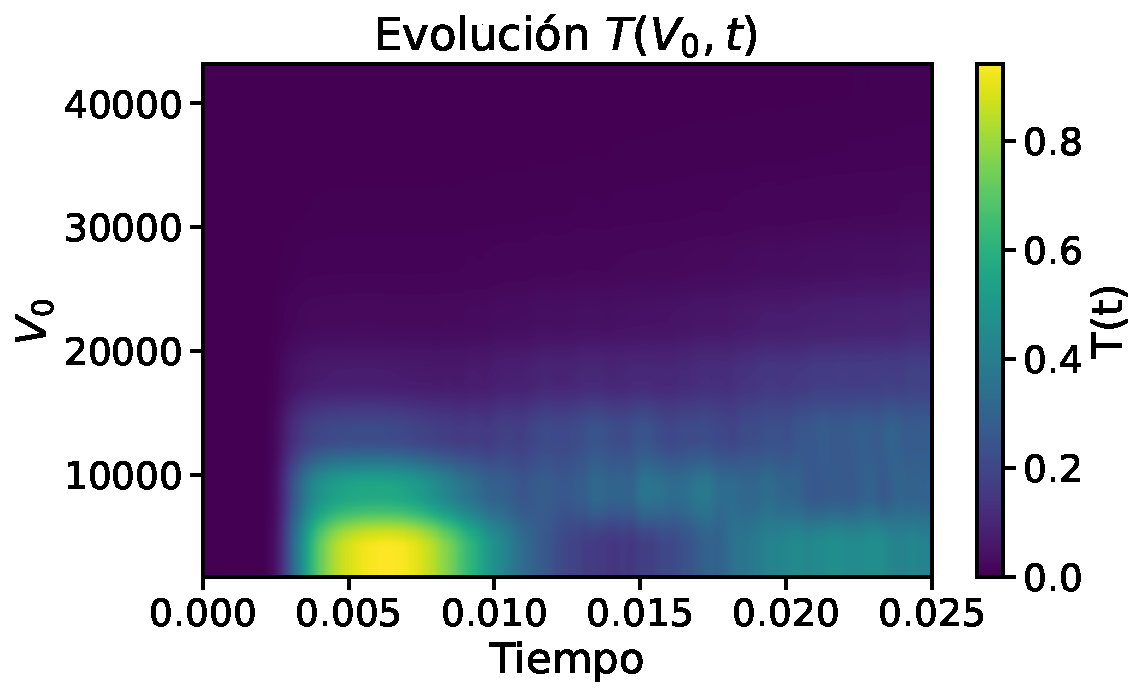
\includegraphics[width=\textwidth]{figures/mapa_T_V0.pdf}
        \caption{Evolución $T(V_0,t)$}
        \label{fig:mapa_V}
    \end{subfigure}
    \hfill
    \begin{subfigure}[b]{0.48\textwidth}
        \centering
        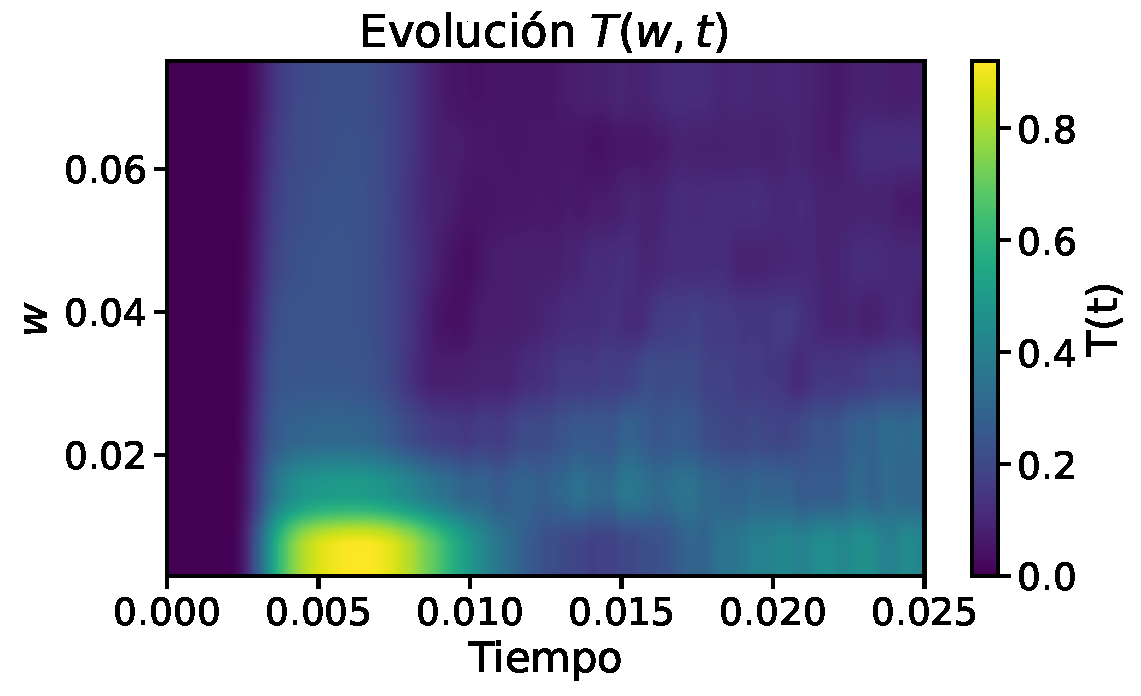
\includegraphics[width=\textwidth]{figures/mapa_T_w.pdf}
        \caption{Evolución $T(V_0,t)$}
        \label{fig:mapa_w}
    \end{subfigure}

    \caption{Mapas 2D que muestran la evolución de la probabilidad de transmisión $T$ en función del tiempo variando $V_0$ (Izquierda) o $w$ (Derecha).}
  \label{fig:mapas}
\end{figure}

Finalmente, la animación de la parte real \(\Re(\psi)\) (Figura \ref{fig:real_part}) muestra la conservación de coherencia de fase durante todo el proceso de dispersión. Las oscilaciones espaciales preservan continuidad incluso tras la separación entre componentes transmitidas y reflejadas, evidenciando que el fenómeno de túnel no puede interpretarse como una transición clásica estocástica, sino como la evolución determinista de un estado cuántico coherente distribuido espacialmente.


\begin{figure}[h!]
    \centering
    \href{https://youtu.be/frQ7Apgdps4}{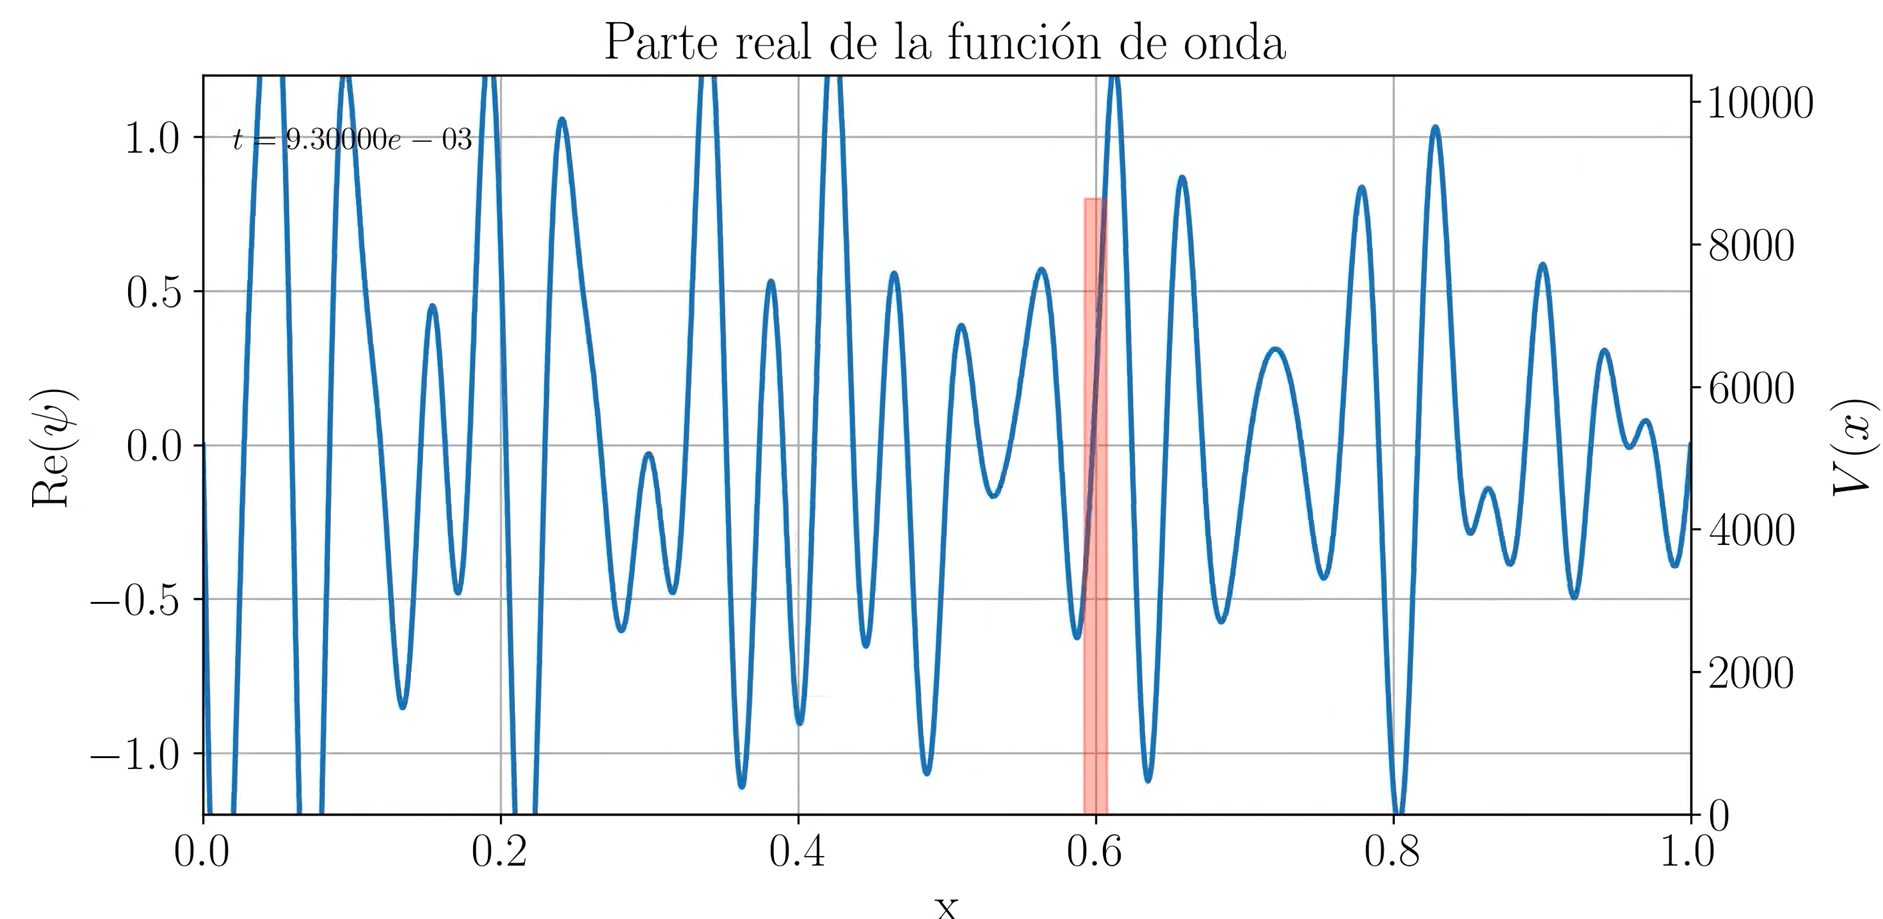
\includegraphics[width=0.75\linewidth]{figures/real_part.png}}
    \caption{Evolución temporal de la parte temporal un paquete gaussiano incidente sobre una barrera rectangular de potencial en el régimen $V_0>E$. Animación completa disponible en \href{https://youtu.be/frQ7Apgdps4}{YouTube}.}
    \label{fig:real_part}
\end{figure}

% ---------------------------------------------------------
% 1. Experimento de Doble Rendija
% ---------------------------------------------------------


\subsection{Resultados y Análisis: Simulación de Doble Rendija}

La visualización temporal detalla la evolución de un paquete de ondas incidente que se propaga hacia un obstáculo situado en $x = 0 $. Antes de la colisión (zonas de $x \approx -20 \, a_0$), la función de onda exhibe un frente de fase coherente. Al atravesar las rendijas, el haz experimenta difracción radial, conformando un patrón de franjas de interferencia. La escala cromática parametriza la fase (o argumento) de la función de onda compleja, variando estrictamente en el dominio $\arg(\psi) \in [-\pi, \pi]$.


\begin{figure}[h!]
    \centering
    \href{https://youtube.com/shorts/XPvwuIbuQ5A?feature=share}{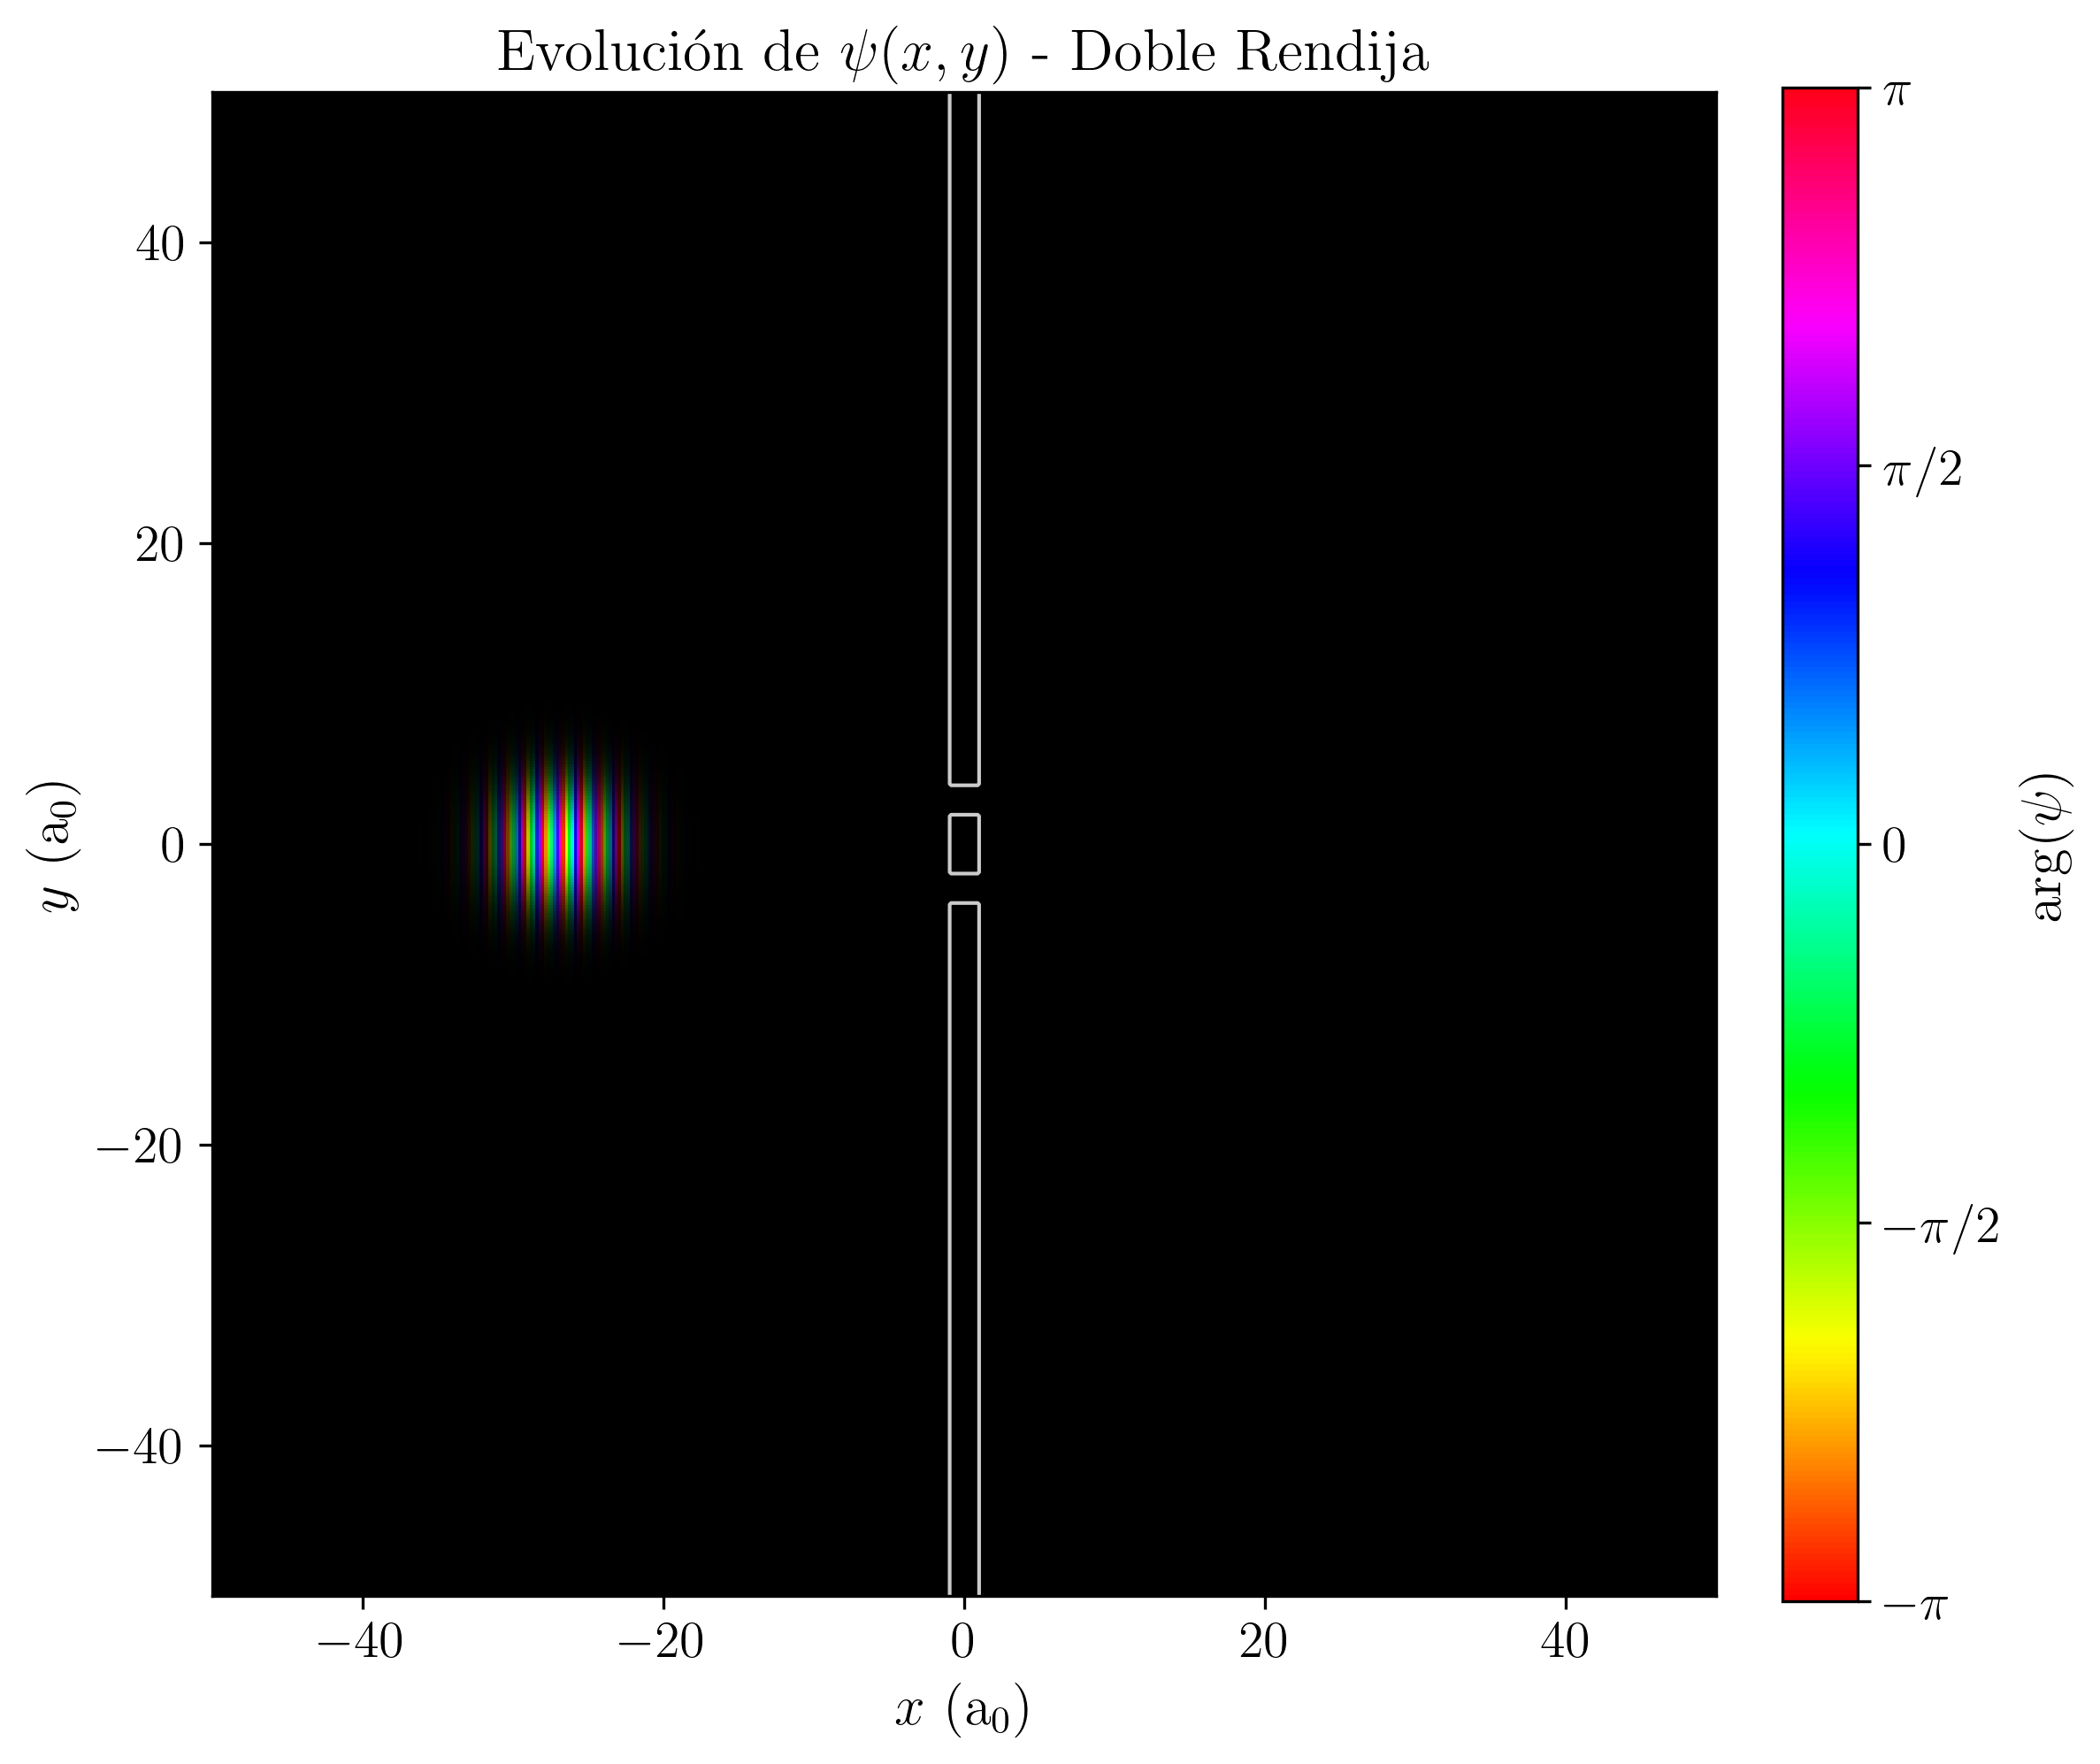
\includegraphics[width=0.65\linewidth]{figures/doble_rendija.png}}
    \caption{Experimento de la Doble Rendija. Animación completa en \href{https://youtube.com/shorts/XPvwuIbuQ5A?feature=share}{YouTube}}
\end{figure}

El comportamiento espaciotemporal registrado es una manifestación fenomenológica explícita de la ecuación de Schrödinger dependiente del tiempo. La emergencia de un patrón de franjas posterior a $x = 0 $ confirma la naturaleza ondulatoria y el principio de superposición cuántica. Las transiciones topológicas de coloración (de $-\pi$ a $\pi$) acopladas a nodos de amplitud nula revelan la interferencia destructiva, lo cual atestigua la conservación de la coherencia de fase del estado cuántico tras la bipartición espacial del haz original.

% ---------------------------------------------------------
% 2. Estructura Atómica del Nanografeno
% ---------------------------------------------------------

\subsection{Resultados y Análisis: Difracción de Nanografeno (HBC)}

A continuación, se presentan y analizan los resultados obtenidos de la simulación numérica del experimento de difracción de campo lejano utilizando moléculas de nanografeno (Hexa-peri-benzocoroneno, HBC) como frentes de onda coherentes. El análisis abarca desde la caracterización de la estructura de la muestra en el espacio real hasta la interpretación de los patrones de interferencia resultantes.

\subsubsection{Caracterización de la Muestra en el Espacio Real}
La Figura \ref{fig:estructura_hbc} proporciona un mapeo coordenado detallando la arquitectura atómica del nanografeno (HBC) utilizado como rejilla de difracción. A diferencia de un conglomerado de moléculas aisladas, este clúster molecular se compone de una red densa de siete anillos hexagonales aromáticos fusionados, donde los anillos periféricos comparten enlaces carbono-carbono con el anillo central.

\begin{figure}[h!]
    \centering
    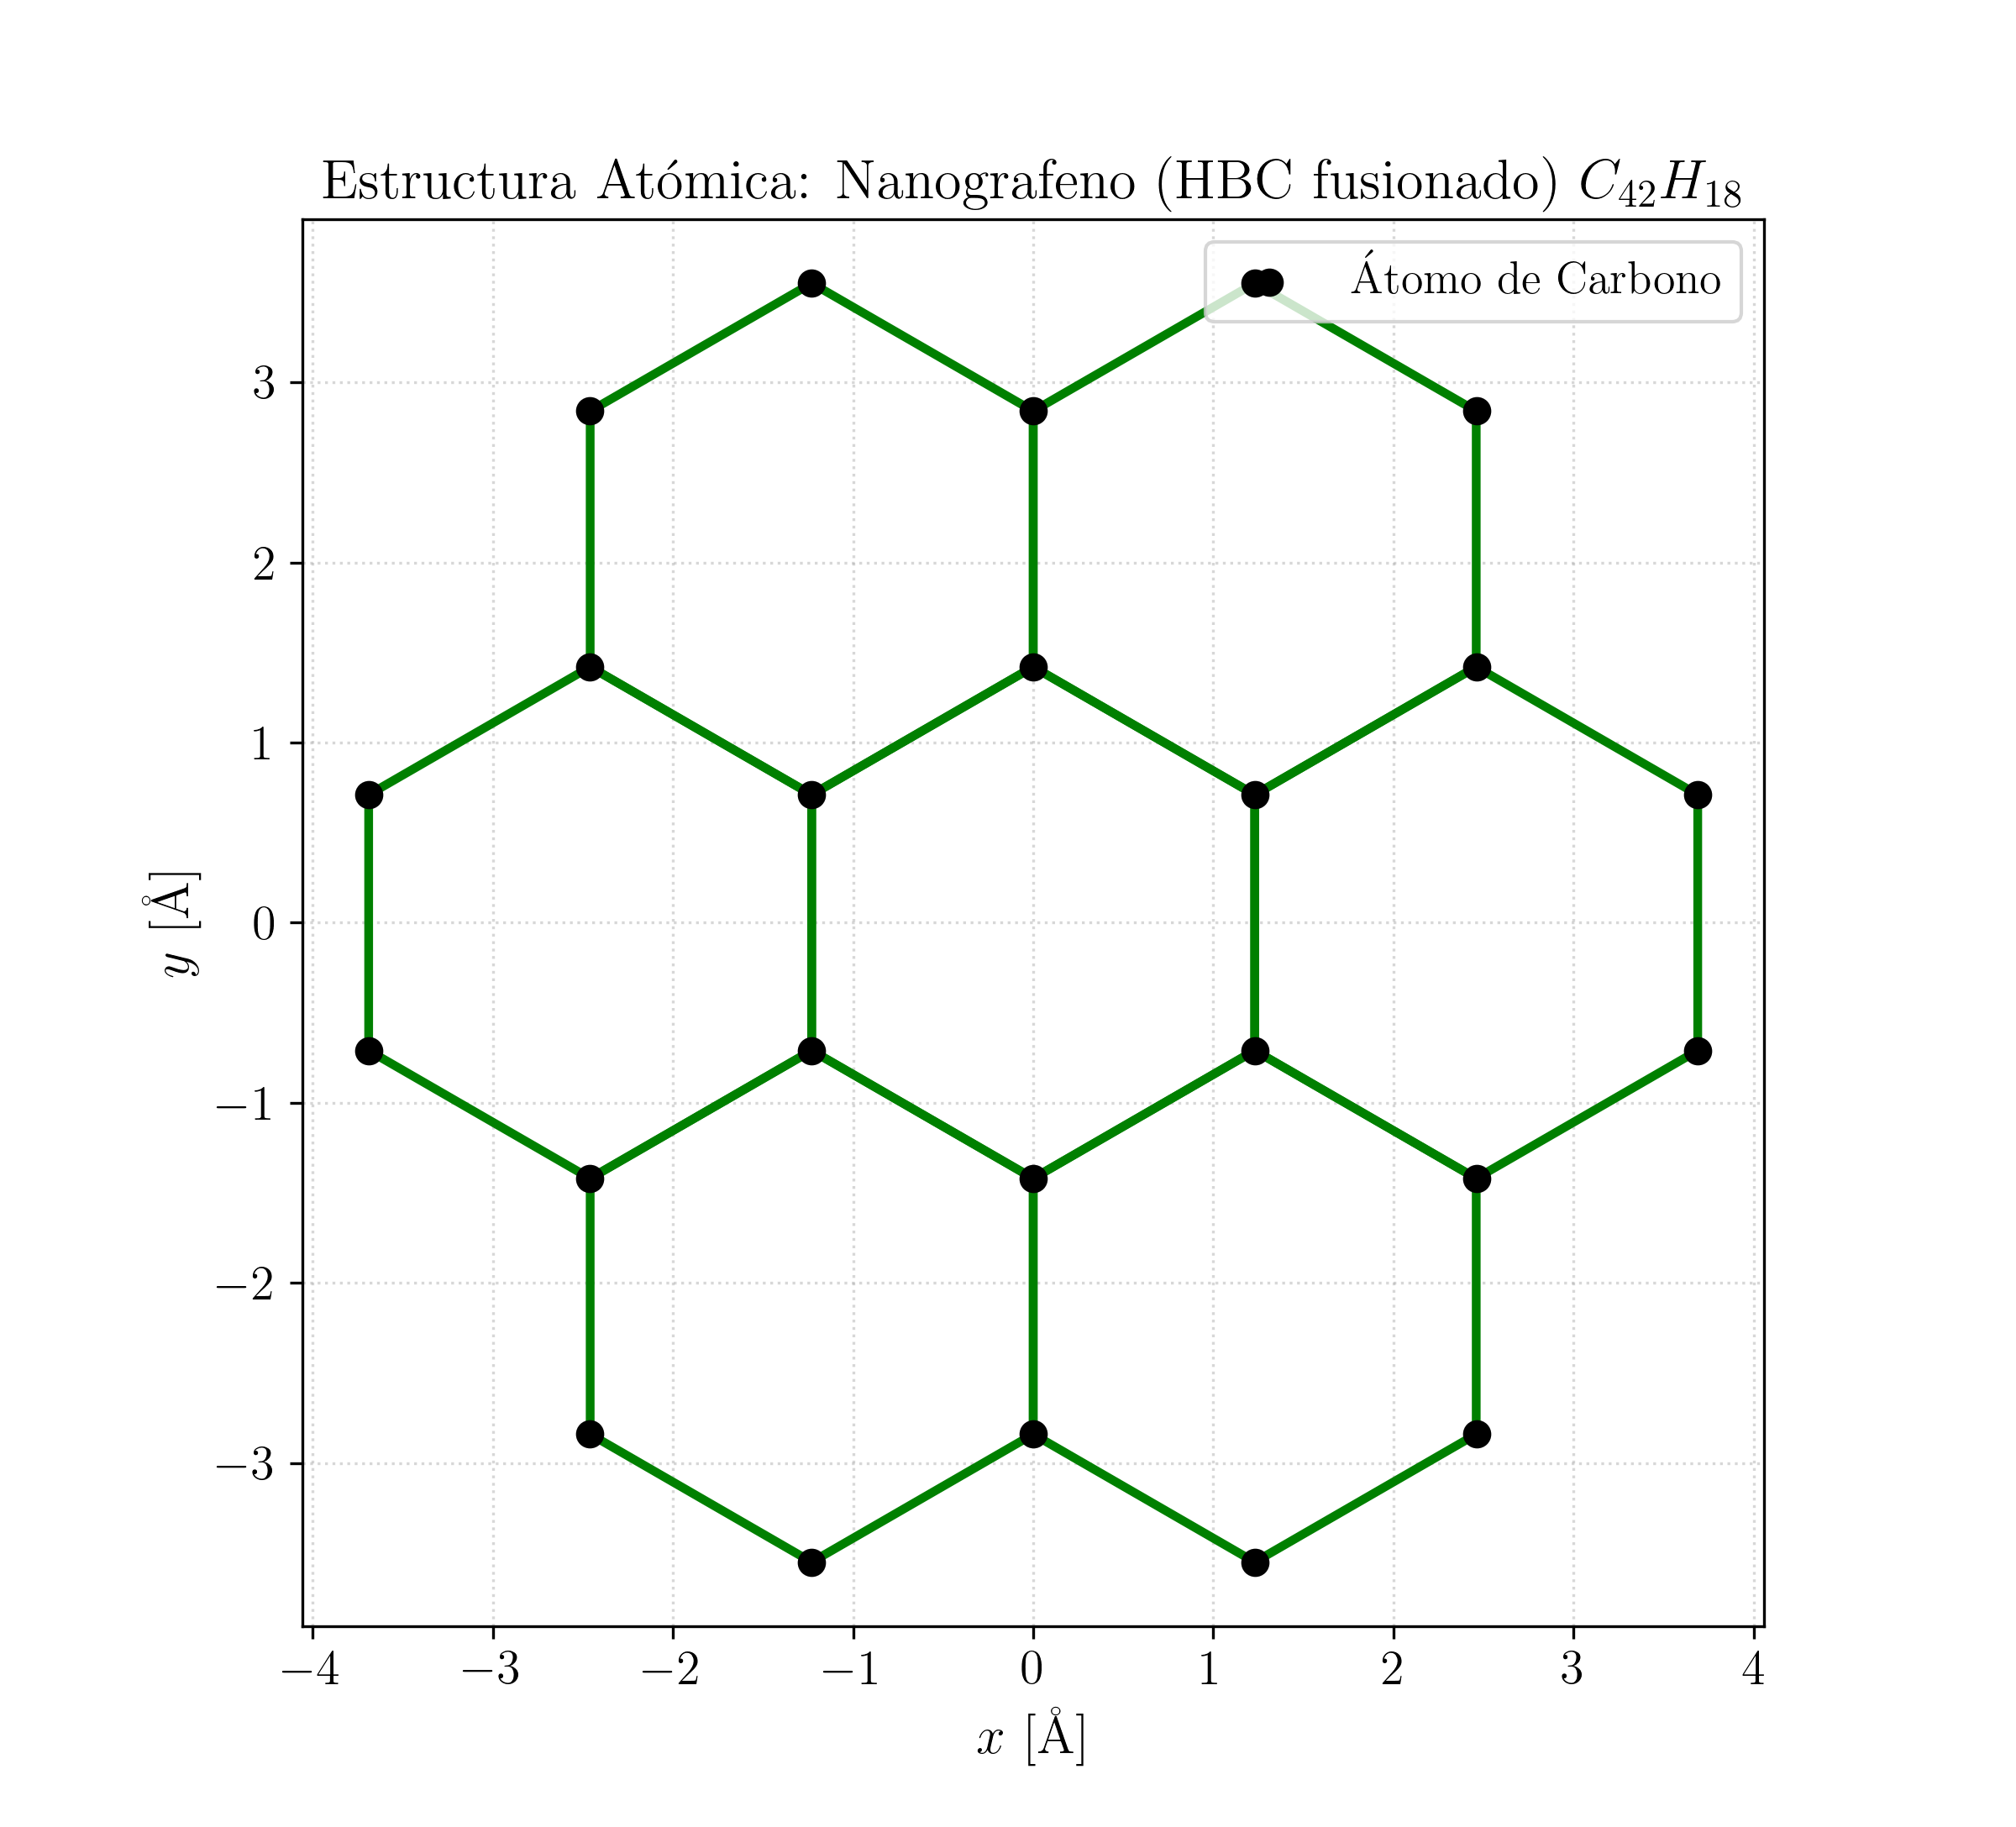
\includegraphics[width=0.5\textwidth]{figures/estructura_atomica_nanografeno_fused.png}
    \caption{Disposición geométrica fusionada de la red en el espacio real para la molécula de Hexa-peri-benzocoroneno ($C_{42}H_{18}$). Los puntos negros representan los 42 átomos de carbono únicos y las líneas verdes los enlaces covalentes compartidos.}
    \label{fig:estructura_hbc}
\end{figure}

Las coordenadas están proyectadas en unidades de angstroms (\AA) para ambos ejes. El entramado atómico se extiende en una región espacial de aproximadamente $-5 \, \text{\AA}$ a $5 \, \text{\AA}$ en el eje transversal ($x$) y de $-5 \, \text{\AA}$ a $5 \, \text{\AA}$ en el eje vertical ($y$), evidenciando una distancia de enlace C-C consistente de $1.42 \, \text{\AA}$ en toda la topología fusionada.

% La estricta periodicidad hexagonal y la naturaleza fusionada de los anillos manifiestan la hibridación orbital $sp^2$ intrínseca de los sistemas aromáticos policíclicos de carbono. Esta macro-molécula plana exhibe un grupo de simetría puntual $D_{6h}$. Identificar con alta precisión este arreglo espacial y su densidad electrónica $\rho(\mathbf{r})$ es un prerrequisito analítico fundamental, ya que su Transformada de Fourier dictaminará las direcciones permitidas de dispersión constructiva en el espacio recíproco.

% ------------------------------------------------------------------------------
% SUB-SUBSECCIÓN: DINÁMICA DE PROPAGACIÓN
% ------------------------------------------------------------------------------
\subsubsection{Dinámica de Propagación y Acumulación de Intensidad}

La visualización de la dinámica de las moléculas desde la rejilla hasta la pantalla se presenta mediante una animación (Figura \ref{fig:animation_scat}).



\begin{figure}[H]
    \centering
\href{https://youtu.be/2b96mZdyjBI}{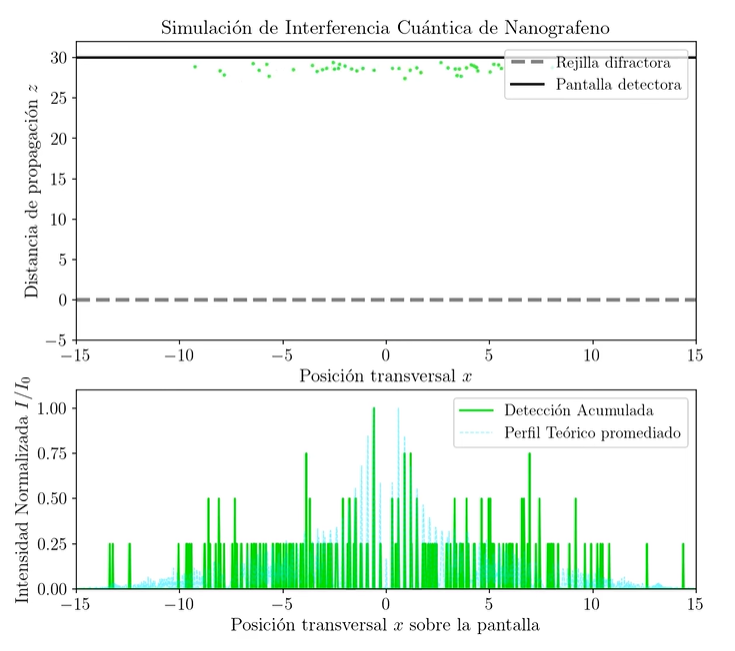
\includegraphics[width=0.7\linewidth]{figures/animation_thumbnail.png}}
    \caption{Instantánea de la animación de simulación. Panel superior: Propagación de las moléculas (puntos verdes) en el espacio $x-z$. El panel inferior muestra la evolución del histograma de detección transversal ($I/I_0$) en la pantalla ($z=30$) a medida que se acumulan eventos. Animación disponible en \href{https://youtu.be/dHB0DgZWk-c}{YouTube}.}
    \label{fig:animation_scat}
\end{figure}

La interfaz de resultados muestra dos paneles acoplados temporalmente. El panel superior constata la propagación longitudinal de las moléculas a lo largo del eje $z$, desde la rejilla difractora ($z=0$) hasta la pantalla situada en $z = 30$, mostrando la expansión transversal del haz. Paralelamente, el panel inferior reporta el perfil de intensidad relativa ($I/I_0$) en función de la coordenada transversal $x \in [-15, 15]$. Se identifica un pico principal o lóbulo central en $x = 0$ con convergencia máxima de $I/I_0 = 1.0$, flanqueado por picos secundarios sinusoidales amortiguados. Se observa un solapamiento casi directo entre la curva de la ``Detección Acumulada'' (puntos muestreados aleatoriamente) y el ``Perfil Teórico promediado'' (curva cian).

La máxima amplitud registrada en el origen corresponde al orden de difracción $0$, representativo del volumen de la onda no dispersada. Las oscilaciones paramétricas colindantes son el resultado directo de la interferencia constructiva de múltiples rendijas (factor de estructura) impuesta por la red atómica de la muestra de HBC. La convergencia del histograma de partículas hacia el modelo teórico certifica la validez estadística de la simulación de Monte Carlo y confirma que el montaje operó bajo condiciones de alta coherencia longitudinal, permitiendo la resolución de picos de interferencia de alto orden.

% ------------------------------------------------------------------------------
% SUB-SUBSECCIÓN: PATRÓN 2D
% ------------------------------------------------------------------------------
\subsubsection{Mapeo del Patrón de Interferencia Bidimensional}

Para examinar la simetría del patrón de difracción en todo el plano de detección, se generó un mapeo bidimensional de intensidad (Figura \ref{fig:patron_2d}).

\begin{figure}[h]
    \centering
    % Se asume que el archivo '2d_pattern_graphene.png' está en la carpeta 'figures'
    % Este es el nombre exacto generado por el código corregido.
    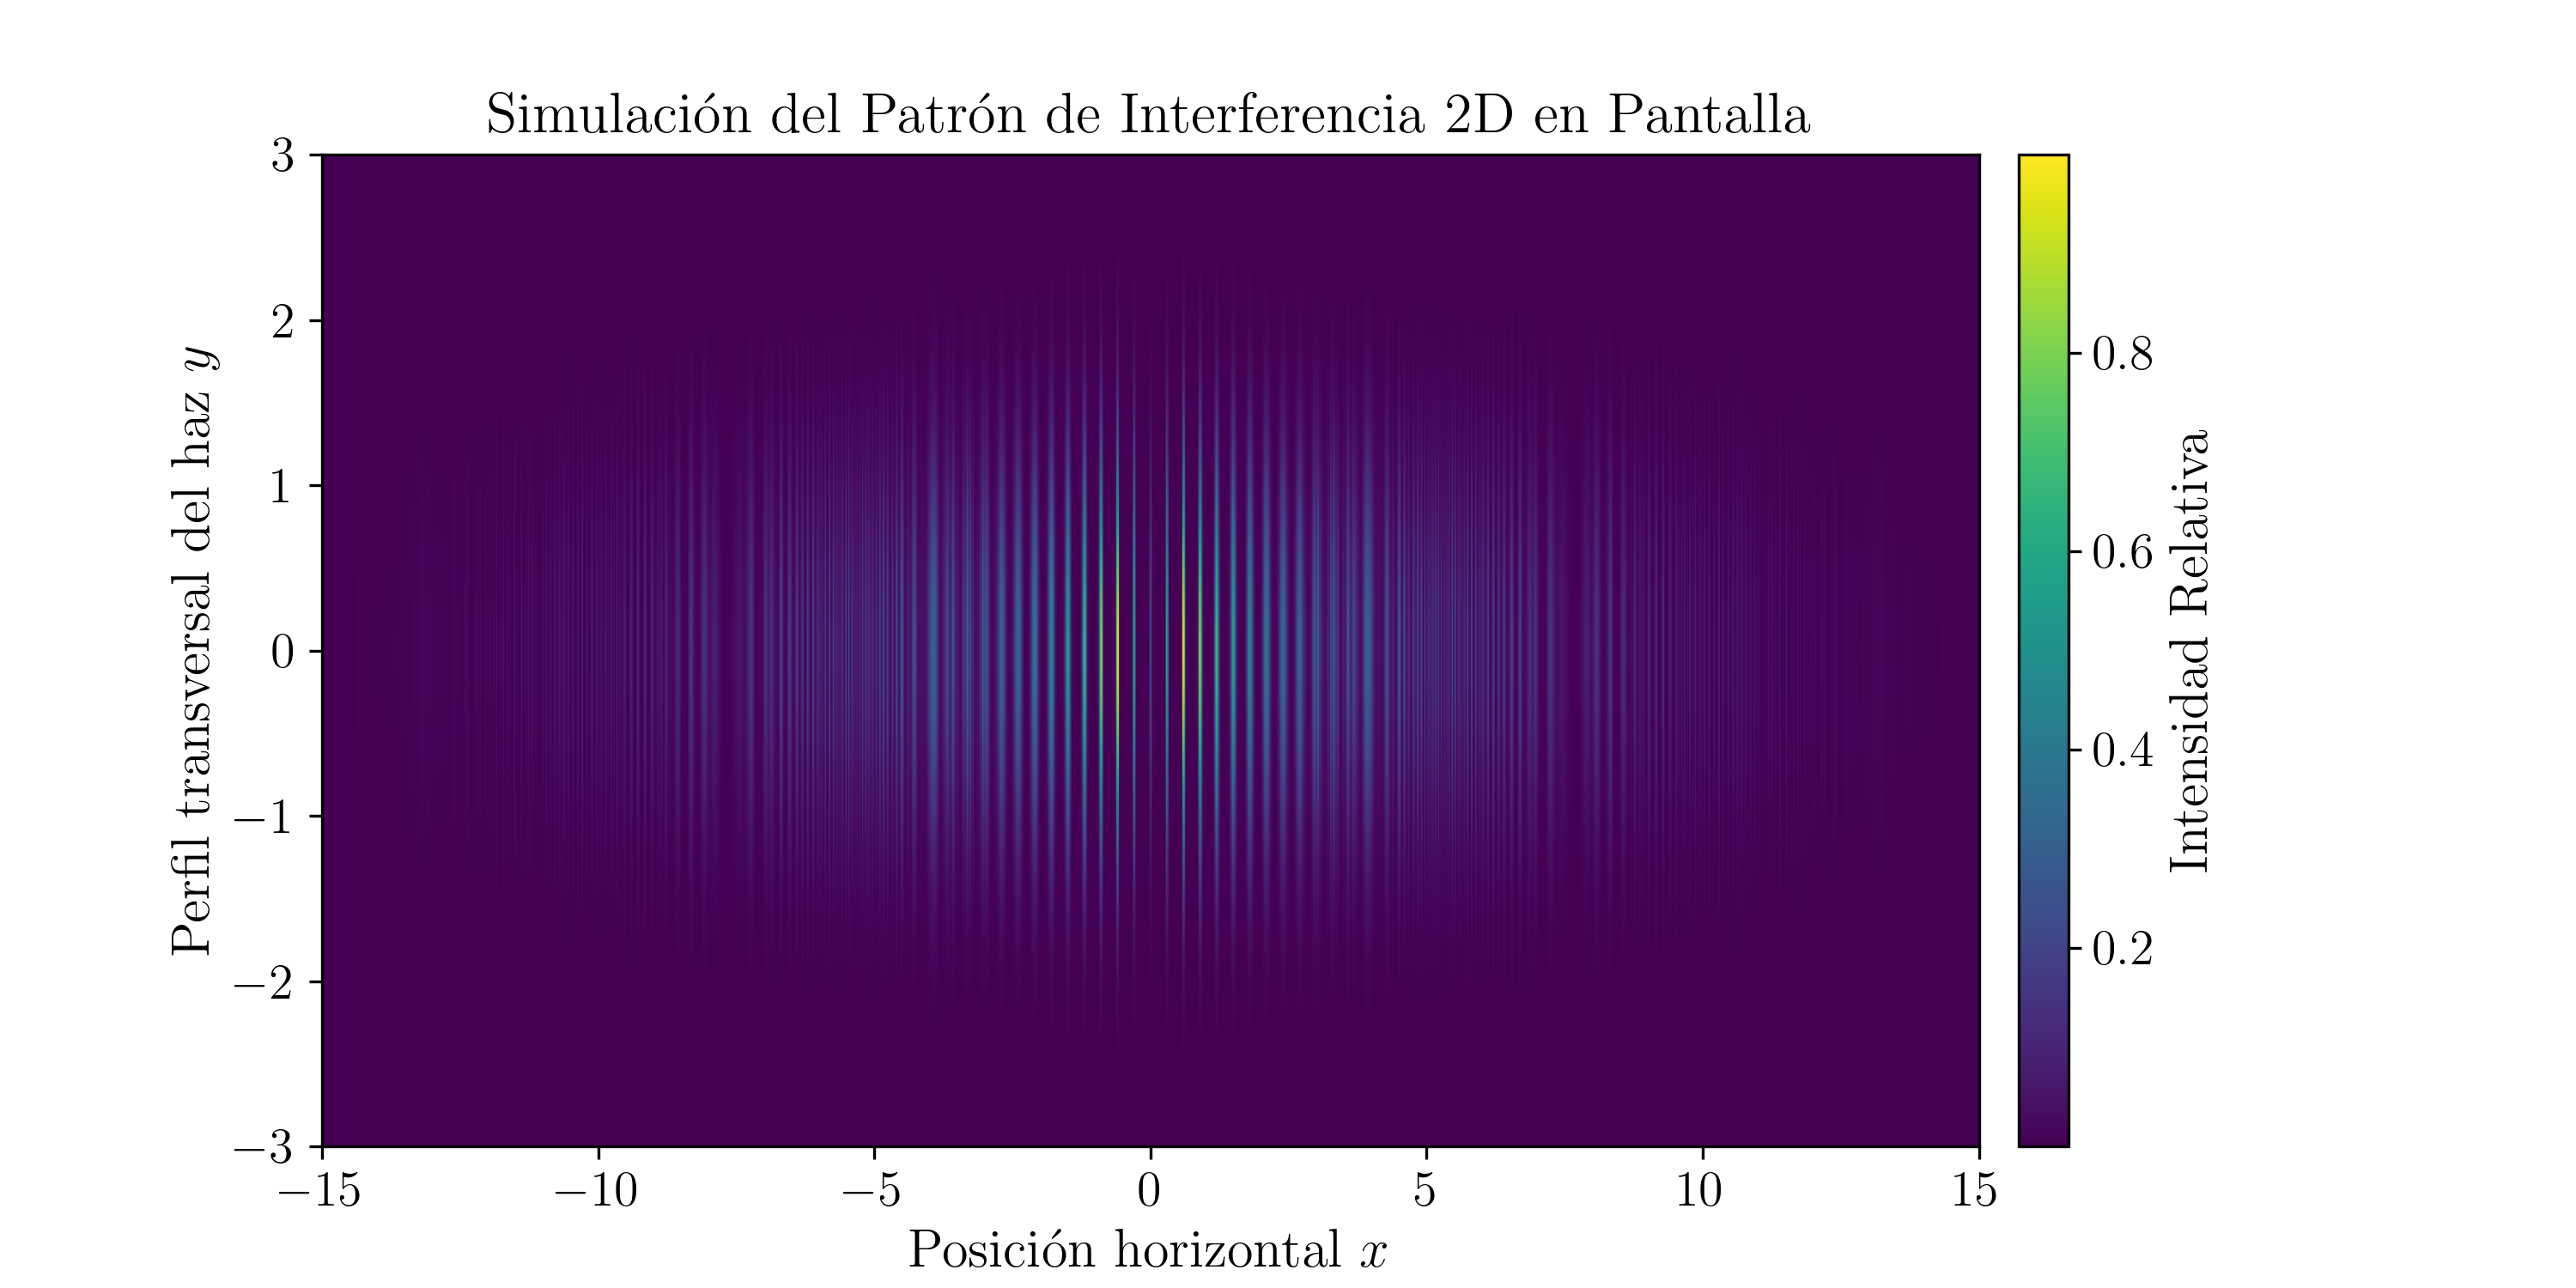
\includegraphics[width=1\textwidth]{figures/2d_pattern_graphene.png}
    \caption{Mapeo bidimensional de intensidad (mapa de calor usando escala 'viridis') para el campo de interferencia de la estructura de nanografeno en la pantalla de detección.}
    \label{fig:patron_2d}
\end{figure}

El gráfico es un mapa de calor  que representa la Intensidad Relativa de Interferencia. Se define el dominio espacial con la Posición horizontal $x \in [-15, 15]$ en el eje de abscisas, cruzada con el Perfil transversal del haz $y \in [-3, 3]$ en las ordenadas. La métrica de color evalúa la intensidad, mostrando una topografía de franjas de difracción verticales densamente empaquetadas. Debido a la envolvente gaussiana simulada en el eje Y para modelar el perfil limitado del haz incidente, la intensidad alcanza sus picos locales máximos en el centro de masa del patrón ($y \approx 0, x \approx 0$), degradándose paulatinamente hacia los bordes periféricos verticales.

Esta visualización codifica la sección eficaz de dispersión coherente mapeada sobre un plano de detección bidimensional en el régimen de Fraunhofer. La marcada anisotropía del patrón (franjas orientadas longitudinalmente) constituye la huella espectral de las restricciones de simetría de la red de HBC fusionado analizada en la Figura \ref{fig:estructura_hbc}. 
% Los máximos de intensidad delimitan los ángulos sólidos que satisfacen la condición de interferencia constructiva de Bragg-Laue, confirmando que la función de onda de prueba fue sensible al arreglo atómico periódico en la escala nanométrica.

% En el dominio 2D, el experimento exhibe visualmente la auto-interferencia macromolecular: el frente de onda continuo se fractura formando lóbulos con fases intercaladas en el eje X, modulados por la intensidad del haz en el eje Y, y separados por líneas nodales de interferencia destructiva estricta.

% Finalmente, la integración del espectro térmico (policromaticidad) en la simulación del nanografeno modela fielmente la realidad experimental. Se constata que la macromolécula actúa como un frente de onda coherente; sin embargo, la dispersión de velocidades provoca que los diferentes regímenes de difracción asociados a cada longitud de onda de de Broglie se solapen. Como resultado visual, el lóbulo central (orden cero) preserva su nitidez geométrica, mientras que los picos de interferencia de orden superior sufren un emborronamiento progresivo hasta fundirse en un continuo incoherente, ratificando la extrema sensibilidad de los sistemas macromoleculares a su entorno térmico longitudinal.